This section outlines the methodological approach adopted to measure liquidity risk and investors' sentiment, along with their rationale. These factors are integrated into an enhanced asset pricing framework based on the FF5 and C4F. Subsequently, the implementation of the Random Forest (RF) algorithm is detailed. Next, the rule-based model will be extracted from the RF for comparison and application to the Association Rule Learning Sector Rotation Strategy. Decades of empirical work show that both liquidity risk and investor sentiment earn distinct premiums that the tradidional FF5 and C4F factors cannot fully capture. Stocks with high liquidity betas command an extra return even after controlling for size, value, and momentum \citeA{pastor_2003,acharya_2005}, while sentiment indices systematically predict the mispricing of speculative stocks \citeA{baker_2006,stambaugh_2015}. By bringing these factors into asset pricing models, this paper aim to (i) close the explanatory gaps left by traditional linear models, (ii) supply economically viable factors for the subsequent RF framework, and (iii) test whether richer factor information translates into superior sector-rotation signals. 

\subsection{Factor enhancements}
\subsubsection{Liquidity Risk factors}

The construction of liquidity factors closely aligns with the methodology outlined by \citeA{gu_2020}. The authors include a suite of seven stock level liquidity proxies: turnover and turnover volatility (\texttt{turn}, \texttt{SDturn}), log market equity (\texttt{mvel1}), dollar volume (\texttt{dolvol}), Amihud illiquidity (\texttt{ILLQ}), number of zero trading days (\texttt{zerotrade}), and bid-ask spread (\texttt{baspread}). Turnover measures trading liquidity:

\begin{equation}
\text{turn}_{i,t} = \frac{\text{Number of shares traded}}{\text{Number of outstanding shares}}
\end{equation}

While its standard deviation (\texttt{SDturn}) captures episodic illiquidity shocks (stocks with infrequent or highly variable trading demand higher expected returns as compensation). Log market equity (\texttt{mvel1}) and dollar volume (\texttt{dolvol}) proxy for firm size and the how active the market is, respectively, since smaller firms and low-\texttt{dolvol} issues exhibit thinner order-book depth (not a lot of people are buying and selling). Bid-ask spread (\texttt{baspread}) directly reflects immediacy costs, and a wider spread signals greater liquidity risk. The count of zero-trading days (\texttt{zerotrade}) quantifies outright market "gaps" where trading is impossible (your equity literally cannot be liquidated), each gap intensifying illiquidity premia. Finally, Amihud's \texttt{ILLQ} is defined as:
\begin{equation}
\label{eq:amihud}
\text{ILLIQ}_{i,y}
=
\frac{10^6}{D_i^y}
\sum_{d=1}^{D_i^y}
\frac{\lvert R_{i,d}\rvert}{\text{VOL}_{i,d}}
\end{equation}

Here, $D_i^y$ denotes the total number of trading days for which data are available for stock $i$ during year $y$, $R_{i,d}$ is the daily return on trading day $d$, computed as the percentage change in closing price from the previous day. $\text{VOL}_{i,d}$ is the dollar trading volume on that same day. The ratio $\lvert R_{i,d}\rvert/\text{VOL}_{i,d}$ captures the price impact per dollar traded, and averaging over all $D_i^y$ days yields the annual illiquidity estimate. However, since the data in this thesis is collected on a daily basis, this illiquidity measure is calculated with $D_i^y = 1$. By including proxies for trading frequency, volume scale, price impact, cost of immediacy, and market “holes,” \citeA{gu_2020} ensure that no single dimension of illiquidity is overlooked.Empirical tests have confirmed that different measures emerge as top predictors of future returns in varying market environments.

\subsubsection{Sentiment factors}
%% OUTLINE: wurgler -> antoniu -> XU enhanced
\citeA{wurgler_2006} constructed a sentiment index (BW index hereafter) by capturing the principal components within six proxies: closed-end fund discount (\texttt{CEFD}), NYSE share turnover (\texttt{turn}), the number and average first-day returns of IPOs (\texttt{NIPO, RIPO} respectively), equity share in new issues (\texttt{S}) and dividend premium (\texttt{P}). \footnote{However, by March 2016, the NYSE share turnover proxy has been dropped in the database due to "the explosion of institutional high-frequency trading and the migration of trading to a variety of venues" \cite{ung_2023}}

First, all the raw proxy is standardized into a principal component analysis (PCA). The first principal component of this first stage PCA captures the common sentiment factor over time. Next, for each of the six proxies, \citeA{wurgler_2006} examines which of its own current or lagged series has the highest correlation with that first stage index, and then re-runs a second PCA on just those six selected series to distill their shared. Finally, the resulting six PCA loadings are rescaled so that the index has unit variance, yielding the coefficients reported in the following equation:
\begin{equation}
    \label{eq:sentiment}
    \begin{split}
    \text{SENTIMENT}_t = -0.241\,\text{CEFD}_t + 0.242\,\text{TURN}_{t-1} \\ + 0.253\,\text{NIPO}_t 
    + 0.257\,\text{RIPO}_{t-1} \\ + 0.112\,S_t - 0.283\,P^{D-ND}_{t-1} , 
    \end{split}
\end{equation}

where each proxy has been standardized. $\text{D}-\text{ND}$ is the difference between dividend payers and non-dividend payers. Principal Component Analysis(PCA) reveals the hidden common factor from this group of factors by transforming the data into principal components (PCs) that would capture as much variance in the data as possible. PC1 should capture the maximum variation from the sentiment proxies, thereby serving as an aggregate measure of investor sentiment. Since both market sentiment and the business cycle can drive common variation in financial data, the PCA will treat both as sources of variance without distinguishing whether that variance comes from changes in investor sentiment or broader macroeconomic factors. A second orthogonalized index is formed by regressing each proxy \(X_{i,t}\) on business-cycle controls \(Z_t\). In this regression, the residuals \(\epsilon_{i,t}\) is orthogonal (uncorrelated) with \(Z_t\), which isolates the variation in \(X_{i,t}\) independent of macroeconomic fluctuations.
Specifically, we estimate
\begin{equation}
X_{i,t} = \alpha_i + \boldsymbol{\gamma}_i'\mathbf{Z}_t + \epsilon_{i,t},
\end{equation}
where \(\mathbf{Z}_t\) includes quarterly GDP growth, industrial production growth, the unemployment rate, and the Treasury term spread. The resulting residuals \(\epsilon_{i,t}\), denoted \(X_{i,t}^\perp\), capture the component of each proxy orthogonal to macroeconomic fluctuations and serve as the ‘pure’ sentiment measure. Equation \ref{eq:sentiment_orth} presents the orthogonalized sentiment index, with the superscript \(\perp\) indicating the removal of business-cycle effects. The coefficients of this equation are calculated in the same way as \cref{eq:sentiment}.

\begin{equation}
    \label{eq:sentiment_orth}
    \begin{split}
    \text{SENTIMENT}^{\perp}_t = &-0.198\,\text{CEFD}^{\perp}_t + 0.225\,\text{TURN}^{\perp}_{t-1} \\
    &+ 0.234\,\text{NIPO}^{\perp}_t + 0.263\,\text{RIPO}^{\perp}_{t-1} \\
    &+ 0.211\,S^{\perp}_t - 0.243\,\text{P}^{\text{D} - \text{ND},\perp}_{t-1}
    \end{split}
\end{equation}


However, \citeA{ung_2023} pointed out several problems with the BW index. First, though it has robust predictive perfomance on a cross- sectional level, it is weak for aggregate market retuerns in time series regressions. Even \citeA{wurgler_2007} pointed this out themselves in the paper. Second, the BW index assumes that the contributions of each sentiment proxy to the aggregate index are fixed over time. Finally, the index has `look ahead bias': PCA uses the whole sample, and forecasts at time $t$ should not rely on data that would only become available after $t$. Therefore, \citeA{ung_2023} constructed an enhanced index to address these problems. The time-varying BW sentiment index ($S^{TV}$ hereafter) is constructed on a three years rolling window basis to use the most up-to-date information at each $t$, and is built upon \cref{eq:sentiment_orth}. This rolling window allows the model to adjust to structural breaks in the market without distorting the sentiment index. Furthermore, adjustments to the sign of the RICO proxy display a negative initial loading. This paper will use \citeA{ung_2023} $S^{TV}$ index to measure investors' sentiment.

In addition to the Enhanced BW index, the Daily News Sentiment Index from the Federal Reserve Bank of San Francisco provides a high-frequency gauge of U.S. economic sentiment, capturing short-run fluctuations in public perceptions as reported by major national newspapers. Specifically, the index aggregates sentiment scores derived from economics-related articles in 24 leading U.S. newspapers, including those with nationwide reach such as the \emph{New York Times} and the \emph{Washington Post}. Articles included in the measure must contain at least 200 words and be classified by Factiva (a news aggregator) as relating to "economics" and the "United States". To generate the sentiment score, \citeA{shapiro_2020} combine general purpose sentiment dictionaries with a custom lexicon to more accurately reflect the tone and context of economic reporting. Sentiment is scored at the article level and then aggregated using a trailing weighted average, in which more recent articles receive higher weights, with geometric decay over time. This method makes sure that any adjustments for potential shifts in the composition of the newspapers within the index is accounted for.

Complementing the two official sentiment indexes, this paper also utilizes a proxy for sentiment, the Volatility Index (VIX hereafter) by \citeA{vix_cboe}. The VIX, commonly reffered to in the finance sector as the 'fear index' computes a 30 day forward-looking estimate of market volatility by aggregating the prices of out-of-the-money S\&P 500 index options, weighted across a broad range of strike prices and interpolated to produce a constant maturity of 30 days. It uses both put and call options with expirations between 23 and 37 days, along with current U.S. Treasury rates, to accurately reflect current market expectations. The formula essentially replicates a theoretical variance swap by summing the contributions from each eligible option then takes the square root and annualizes the result. The formula for VIX is as follows:
\begin{equation}
    \label{eq:vix}
    \text{VIX} = 100 \times \sqrt{\frac{2}{T} \sum_i \frac{\Delta K_i}{K_i^2} e^{RT} Q(K_i) - \frac{1}{T} \left(\frac{F}{K_0} - 1\right)^2}
\end{equation}

where $T$ is time to expiration, $F$ is the forward index level derived from index option prices, $K_0$ is the first strike below $F$, $K_i$ is the strike price of the $i$th out-of-money option, $\Delta K_i$ is the interval between strike prices, $R$ is the risk-free interest rate to expiration, and $Q(K_i)$ is the midpoint of the bid-ask spread for each option with strike $K_i$.

With this information, this thesis will add the Enhanced BW index, daily news sentiment index, and VIX as the sentiment proxies to the C4F and FF5 models.

\subsection{Model training and its enhancements}

Each model specification is estimated across four variations—C4F only, FF5 only, C4F + liquidity + sentiment, and FF5 + liquidity + sentiment—and applied to each of the 11 sectors over the 1998-2017 in-sample period, with 2018 reserved for out-of-sample evaluation. All performance metrics and model coefficients reported are from the models trained within 1998-2017. Model performance is assessed using three standard metrics.  First, the coefficient of determination (R-squared) is defined as  
\begin{equation}
\label{eq:rsquared}
R^2 \;=\; 1 \;-\; \frac{\sum_{t=1}^{T}\bigl(y_{t}-\hat y_{t}\bigr)^2}{\sum_{t=1}^{T}\bigl(y_{t}-\bar y\bigr)^2},
\end{equation}  
where \(y_t\) denotes the observed return, \(\hat y_t\) the model prediction, \(\bar y = T^{-1}\sum_{t=1}^T y_t\), and \(T\) is the number of observations in the sample.  To adjust for differing numbers of predictors \(p\), we compute the adjusted \(R^2\):  
\begin{equation}
\label{eq:adjrsquared}
\mathrm{Adj}\,R^2 \;=\; 1 \;-\; \bigl(1 - R^2\bigr)\,\frac{T - 1}{T - p - 1}.
\end{equation}  

We also compute the mean absolute error:
\begin{equation}
\label{eq:mae}
\mathrm{MAE} \;=\; \frac{1}{T}\sum_{t=1}^{T}|y_{t}-\hat y_{t}|.
\end{equation}

Finally, predictive accuracy is summarized by the root-mean-square error:  
\begin{equation}
\label{eq:rmse}
\mathrm{RMSE} \;=\; \sqrt{\frac{1}{T}\sum_{t=1}^{T}\bigl(y_{t}-\hat y_{t}\bigr)^2}.
\end{equation}  


Each of these metrics is computed separately for the in-sample period (1998-2017) and the out-of-sample year of 2018 to gauge both explanatory power and true predictive performance. Unlike \citeA{simonian_2019}, the data in this paper is daily, therefore the implementation of the paper's method is on a daily basis instead of monthly. All of the model variations in this section are used to forecast the one day ahead return of each individual sector in 2018. 

\subsubsection{Traditional OLS Factor regression models}
%%%%%%ACTUAL%%%%%%
This thesis will employ two CAPM variants: the C4F of \citeA{cahart_1997} and FF5 of \citeA{ff5_2015}. The following are their respective formulas:

\begin{equation}
    \label{eq:c4f}
    \begin{split}
        R_{i,t} - R_{f,t} &= \alpha_i + \beta_{MKT} (R_{MKT,t} - R_{f,t}) \\
        &\quad + \beta_{SMB} \cdot SMB_t + \beta_{HML} \cdot HML_t \\
        &\quad + \beta_{MOM} \cdot MOM_t + \epsilon_{i,t}
    \end{split}
\end{equation}

\begin{equation}
    \label{eq:ff5}
    \begin{split}
        R_{i,t} - R_{f,t} &= \alpha_i + \beta_{MKT} (R_{MKT,t} - R_{f,t}) \\
        &\quad + \beta_{SMB} \cdot SMB_t + \beta_{HML} \cdot HML_t \\
        &\quad + \beta_{RMW} \cdot RMW_t + \beta_{CMA} \cdot CMA_t + \epsilon_{i,t}
    \end{split}
\end{equation}

where \cref{eq:c4f} is the C4F and \cref{eq:ff5} is the FF5. $R_{i,t}$ is the return on security and $R_{f,t}$ is the risk-free return; which makes $R_{i,t} - R_{f,t}$ is the excess return on a security. $SMB$ (small minus big) is the size factor, capturing the excess returns of small-cap stocks over large-cap stocks, reflecting how higher volatility and growth potential could cause smaller firms to yield higher average returns. $HML$ (high minus low), or the value factor, accounts for the premium earned by stocks with high book-to-market ratios, often associated with underperforming firms that carry higher risk and, consequently, higher expected returns \cite{ff3_1993}. $MOM$ is the one year momentum factor \footnote{In literature, researchers can refer to this factor as PR1YR, UMD (ups minus downs), or WML (winners minus losers.)} \cite{cahart_1997}. In response to \citeA{titman_2004} and \citeA{novymarx_2013} criticisms, two additional factors were added in to the FF3 model \cite{ff5_2015}. $RMW$ (robust minus weak) is the profitability factor, which derives from the empirical observation that firms with higher operating profitability tend to earn higher average returns. $CMA$ (conservative minus aggressive) is the investment factor, which captures the tendency of firms to aggressively invest in new assets, expecting higher returns in the long run. Investors may overpay for such firms due to optimism, which results in lower subsequent returns \cite{titman_2004}.

The empirical analysis will begin by establishing a baseline for each asset pricing variant using time series regressions, employing Ordinary Least Squares (OLS) as outlined by \citeA{simonian_2019}. \cref{eq:c4f} and \cref{eq:ff5}, the two baseline variants will be referred to as C4F-B and FF5-B hereafter. Subsequently, liquidity risk and sentiment indicators will be integrated into these variants, thereby forming an enhanced baseline. The following are the enhanced baseline models:

\begin{equation}
    \label{eq:c4f_expanded}
    \begin{split}
    R_{i,t} - R_{f,t} &= \alpha_i + \beta_{MKT} (R_{MKT,t} - R_{f,t}) \\
    &\quad + \beta_{SMB} \cdot SMB_t + \beta_{HML} \cdot HML_t \\
    &\quad + \beta_{MOM} \cdot MOM_t \\
    &\quad + \beta_{turn} \cdot TURN_{i,t} + \beta_{SDturn} \cdot SDTURN_{i,t} \\
    &\quad + \beta_{mvel1} \cdot MVEL1_{i,t} + \beta_{DOLVOL} \cdot DOLVOL{i,t} \\
    &\quad + \beta_{ILLQ} \cdot ILLQ_{i,t} + \beta{zerotrade} \cdot ZEROTRADE_{i,t} \\
    &\quad + \beta_{baspread} \cdot BASPREAD_{i,t} + \epsilon{i,t}
    \end{split}
\end{equation}

\begin{equation}
    \label{eq:ff5_expanded}
    \begin{split}
    R_{i,t} - R_{f,t} &= \alpha_i + \beta_{MKT} (R_{MKT,t} - R_{f,t}) \\
    &\quad + \beta_{SMB} \cdot SMB_t + \beta_{HML} \cdot HML_t \\
    &\quad + \beta_{RMW} \cdot RMW_t + \beta_{CMA} \cdot CMA_t\\
    &\quad + \beta_{turn} \cdot TURN_{i,t} + \beta_{SDturn} \cdot SDTURN_{i,t} \\
    &\quad + \beta_{mvel1} \cdot MVEL1_{i,t} + \beta_{DOLVOL} \cdot DOLVOL{i,t} \\
    &\quad + \beta_{ILLQ} \cdot ILLQ_{i,t} + \beta{zerotrade} \cdot ZEROTRADE_{i,t} \\
    &\quad + \beta_{baspread} \cdot BASPREAD_{i,t} + \epsilon{i,t}
    \end{split}
\end{equation}

where \cref{eq:c4f_expanded} is the enhanced C4F baseline (C4F-BE) and \cref{eq:ff5_expanded} the enhanced FF5 enhanced baseline (FF5-BE). 



\subsubsection{Random Forest for Regression}

%%%%%%%%OUTLINE%%%%%%%%%%
%Factor models are generally linear. Which kinds of regression are they usally used with (fama macbeth)? 


%%%%%%%%%%ACTUAL%%%%%%%%%%%%%%%
The C4F-B, C4F-BE, FF5-B and FF5-BE, since based on OLS, are linear in nature. These models are favored by finance practitioners because they produce interpretable results. The main results that the practitioners look for is the sensitivities of the factor within the models, or the beta coefficients within the OLS. However, the method is restricted to several assumptions. The features and the target variables of this method are assumed to be linear and the features themselves are not multicollinear. Furthermore, homoskedacity is assumed, where the residuals have constant variance at every level of the features. The residuals should also be independent.

Decision tree based models such as RF offers a more robust and flexible framework.This robustness stems from the model's ensemble approach, which imposes no linearity or homoscedasticity assumptions and thus captures complex nonlinear relationships and interactions that OLS would miss.With regression based problems like asset pricing, decision trees start from a root node and splits into branches. Each branch contains a condition to be full-filled (for example $turn > 10$ or $turn \leq 10$). A tree can have a number of these branches, leading to a complex model that can take into account non-linearity and interactions. The leaf of the decision tree, or the final prediction where the tree does not split further, is a real number that is predicted given all of the previous conditions in the branches are true \cite{cutler_2012}. This method ressembles multiple nested if-then statements, where each if-then statement is a branch of the tree. An example of a decision tree (pruned at depth 3) can be observed in Figure \cref{fig:decision_tree_viz}.

\begin{figure}[H]
    \centering
    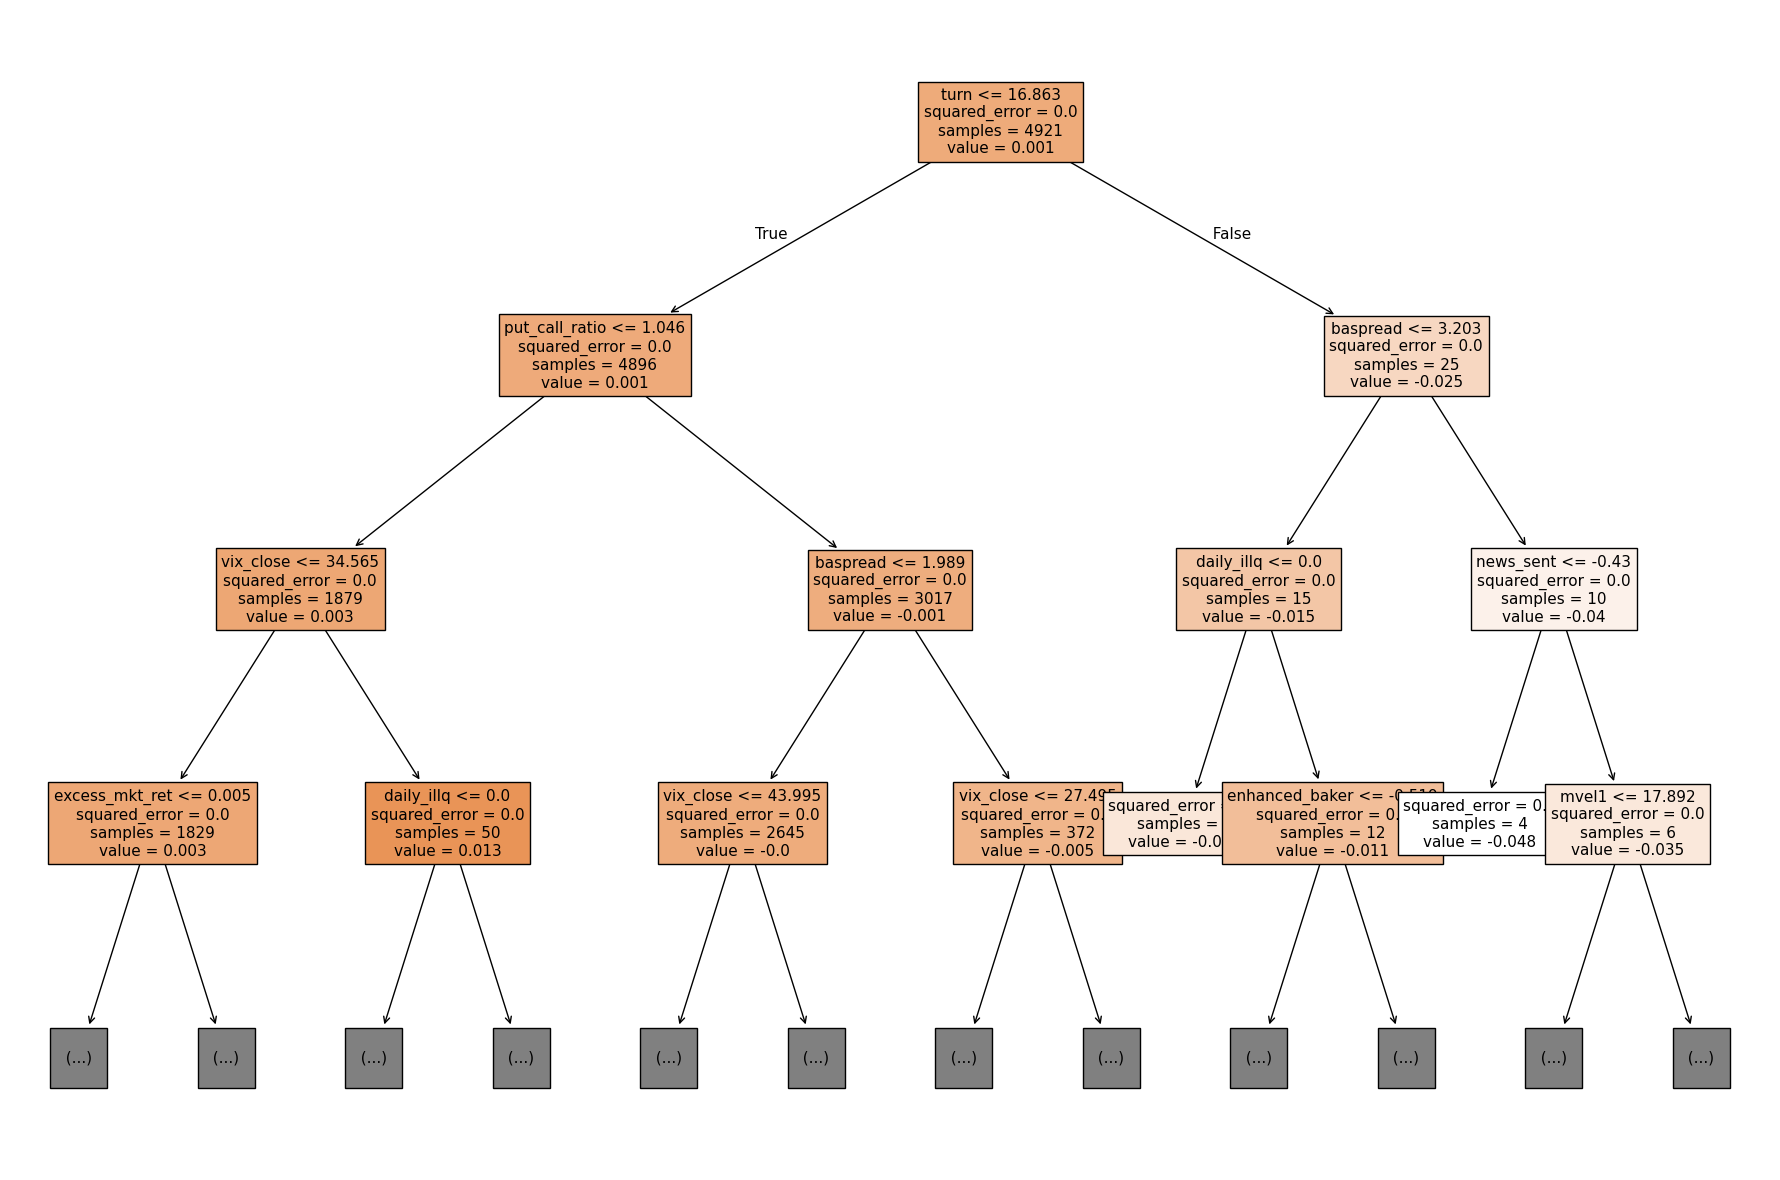
\includegraphics[width=\textwidth]{/Users/minhquangngo/Documents/vsc/erasmus/msc_thesis/latex/plots/methods/tree_example_one.png}
    \caption{Example of a decision tree.}
    \label{fig:decision_tree_viz}
\end{figure}

At its core, a regression tree tries to approximate an unknown regression function by partitioning the $p$-dimensional predictor space  by selecting, at each node, the feature and split point that maximally reduce the squared-error loss. The Classification-And-Regression-Tree (CART) algorithm achieves this with a binary recursive partition procedure that is entirely data driven. The algorithm continues until a stopping criterion is met (for example the leaf size, tree depth,etc.) and each leaf is assigned the mean of all of the observations in that node.

\begin{algorithm}[H]
    \caption{Binary Recursive Partitioning}
    \label{alg:binary_recursive_partitioning}
    
    Let $\mathcal{D} = \{(x_1, y_1), \ldots, (x_n, y_n)\}$ denote the training data, with $x_i = (x_{i,1}, \ldots, x_{i,p})^T$.
    
    \Begin{
        Start with all observations $(x_1, y_1), \ldots, (x_n, y_n)$ in a single node.\;
        
        Repeat the following steps recursively for each unsplit node until the stopping criterion is met:\;
        \Indp
        \Begin{
            Find the best binary split among all binary splits on all $p$ predictors.\;
            Split the node into two descendant nodes using the best split.\;
        }
        \Indm
        
        For prediction at $x$, pass $x$ down the tree until it lands in a terminal node. Let $k$ denote the terminal node, and let $y_{k_1}, \ldots, y_{k_n}$ denote the response values of the training data in node $k$. Predicted values of the response variable for regression are given by $\hat{h}(x) = \bar{y}_k = \frac{1}{n} \sum_{i=1}^n y_{k_i}$\;
    }
    Source: \cite{cutler_2012}
    \end{algorithm}

Random Forests construct a predictive model by aggregating (“bagging”) a large number of decision trees, each of which is grown on a different bootstrap sample of the original data. Bootstrapping means that for each tree, a sample of $N$ observations is drawn with replacement from the training set. This “bootstrap” procedure ensures that each tree sees a slightly different dataset, thereby reducing overall model variance without substantially increasing bias. Moreover, at each split within a tree only a random subset of the available predictors is considered, which further decorrelates the trees and enhances ensemble diversity. Once all trees are grown (usually without pruning), the predictions each tree yields are averaged to yield the final prediction \cite{cutler_2012}. The exact process is outlined in Algorithm \ref{alg:random_forests}. 

A feature of the bootstrap procedure in Random Forests is by sampling with replacement, each tree's training sample could randomly excludes some original observations. These omitted observations are referred to as "out-of-bag" (OOB) samples. For each observation \(i\), one can obtain an OOB prediction \(\hat f_{\mathrm{OOB}}(x_i)\) by averaging the outputs of all trees for which \(i\) was not included in the bootstrap sample. This OOB estimate provides an internal, unbiased measure of predictive performance without the need for a separate validation set. In regression settings, the OOB mean-squared error can be mathematically defined as:
\begin{equation}
\mathrm{MSE}_{\mathrm{OOB}} \;=\; \frac{1}{N}\sum_{i=1}^N\bigl(y_i - \hat f_{\mathrm{OOB}}(x_i)\bigr)^2,
\end{equation}
This metric serves as an efficient proxy for out-of-sample error and can guide hyperparameter tuning (e.g.\ number of trees \(J\), variables per split \(m\), minimum leaf size). Moreover, because each observation is OOB for a different subset of trees, the distribution of OOB residuals is also used to compute variable importance \cite{cutler_2012}. 


\begin{algorithm}[H]
    \caption{Random Forests}
    \label{alg:random_forests}
    
    Let $\mathcal{D} = \{(x_1, y_1), \ldots, (x_N, y_N)\}$ denote the training data, with $x_i = (x_{i,1}, \ldots, x_{i,p})^T$. For $j = 1$ to $J$:
    
    \Begin{
        Take a bootstrap sample $\mathcal{D}_j$ of size $N$ from $\mathcal{D}$.\;
        
        Using the bootstrap sample $\mathcal{D}_j$ as the training data, fit a tree using binary recursive partitioning (Sect. 2.1):\;
        \Indp
        \Begin{
            Start with all observations in a single node.\;
            Repeat the following steps recursively for each unsplit node until the stopping criterion is met:\;
            \Indp
            \Begin{
                Select $m$ predictors at random from the $p$ available predictors.\;
                Find the best binary split among all binary splits on the $m$ predictors from step i.\;
                Split the node into two descendant nodes using the split from step ii.\;
            }
            \Indm
        }
        \Indm
    }
    
    To make a prediction at a new point $x$,
    \Begin{
        $\widehat{f}(x) = \frac{1}{J} \sum_{j=1}^J \widehat{h}_j(x)$
    }
    
    where $\widehat{h}_j(x)$ is the prediction of the response variable at $x$ using the $j$th tree.

    Source: \cite{cutler_2012}
\end{algorithm}

Since the data used in this paper is a time series across 20 years (more about the data used in this paper in Section \ref{sec:data}), we must evaluate model performance in a time dependent context. Hence, we cannot use a simple train-test split. Instead, an extending window approach is used. Concretely, at iteration $t$ the model is trained on observations from time 1 up to $t$, then tested on the hold-out at $t+1$, after which the observation at $t+1$ is appended to the training window for the next evaluation. A visualization of this approach is shown in Figure \ref{fig:extend_win}. Unlike a rolling window split, where the training set maintains a constant size by dropping the oldest observation as the window slides forward, the extending window approach uses the full historical dataset at each step. With this approach, by the time the model is trained on the full dataset, it has seen all the patterns in the data available up to that point. The data that the model is trained on should be stationary (Section \ref{sec:data} shows that excess returns are stationary), otherwise the model will overfit to the noise in the data.

The dataset is divided into 5 sequential train-test folds, with the training window growing by one year at each iteration. This yearly partitioning aligns with the benchmark portfolios of \citeA{ff5_2015}, which are also rebalanced on a yearly basis. Furthermore, based ong previous iterations of this project, it is found that passing 5 train-test fold does not improve on the performance of the model. 

Each test block comprises 212 consecutive trading days (one trading year), with a fixed gap of five trading days between the end of the training window and the start of the evaluation window to avoid look-ahead bias. It balances short-term predictability with realistic transaction-cost assumptions and is widely adopted in recent ML studies of return forecasting \cite{htun_2024}. Introducing a one-week (5-business-day) gap between the folds removes any overlaps between features or labels that span multiple days and the first observations in the test block, eliminating look-ahead bias. This process is called an "Embargo" and is popular in applied quantitative finance Cross Validation workflows \cite{embargo_2020}. %2nd DRAFT: MORE MOTIAVTION WHY?



\begin{figure}[H]
    \centering
    \caption{Extending Window Time Series Cross-Validation}
    \label{fig:extend_win}
    \begin{tikzpicture}[scale=0.8]
        % Define parameters
        \def\totalwidth{12}
        \def\blockheight{0.8}
        \def\spacing{1.2}
        \def\testsize{2}
        
        % Time axis
        \draw[thick, ->] (0, -0.5) -- (\totalwidth + 0.5, -0.5);
        \node[below] at (\totalwidth/2, -1.2) {Time};
        
        % Time labels
        \foreach \i in {0,2,4,6,8,10,12} {
            \draw (\i, -0.4) -- (\i, -0.6);
            \node[below, font=\small] at (\i, -0.6) {t\textsubscript{\i}};
        }
        
        % Split 1
        \node[left] at (-0.5, 4*\spacing) {Split 1:};
        % Training data
        \fill[traincolor] (0, 4*\spacing - \blockheight/2) rectangle (4, 4*\spacing + \blockheight/2);
        \node[white, font=\small\bfseries] at (2, 4*\spacing) {Training};
        % Test data
        \fill[testcolor] (4, 4*\spacing - \blockheight/2) rectangle (6, 4*\spacing + \blockheight/2);
        \node[white, font=\small\bfseries] at (5, 4*\spacing) {Test};
        % Future data
        \fill[futurecolor] (6, 4*\spacing - \blockheight/2) rectangle (\totalwidth, 4*\spacing + \blockheight/2);
        \node[black, font=\small] at (9, 4*\spacing) {Future (unused)};
        
        % Split 2
        \node[left] at (-0.5, 3*\spacing) {Split 2:};
        % Training data (extended)
        \fill[traincolor] (0, 3*\spacing - \blockheight/2) rectangle (6, 3*\spacing + \blockheight/2);
        \node[white, font=\small\bfseries] at (3, 3*\spacing) {Training (Extended)};
        % Test data
        \fill[testcolor] (6, 3*\spacing - \blockheight/2) rectangle (8, 3*\spacing + \blockheight/2);
        \node[white, font=\small\bfseries] at (7, 3*\spacing) {Test};
        % Future data
        \fill[futurecolor] (8, 3*\spacing - \blockheight/2) rectangle (\totalwidth, 3*\spacing + \blockheight/2);
        \node[black, font=\small] at (10, 3*\spacing) {Future (unused)};
        
        % Split 3
        \node[left] at (-0.5, 2*\spacing) {Split 3:};
        % Training data (further extended)
        \fill[traincolor] (0, 2*\spacing - \blockheight/2) rectangle (8, 2*\spacing + \blockheight/2);
        \node[white, font=\small\bfseries] at (4, 2*\spacing) {Training (Further Extended)};
        % Test data
        \fill[testcolor] (8, 2*\spacing - \blockheight/2) rectangle (10, 2*\spacing + \blockheight/2);
        \node[white, font=\small\bfseries] at (9, 2*\spacing) {Test};
        % Future data
        \fill[futurecolor] (10, 2*\spacing - \blockheight/2) rectangle (\totalwidth, 2*\spacing + \blockheight/2);
        \node[black, font=\small] at (11, 2*\spacing) {Future};
        
        % Split 4
        \node[left] at (-0.5, 1*\spacing) {Split 4:};
        % Training data (maximum extension)
        \fill[traincolor] (0, 1*\spacing - \blockheight/2) rectangle (10, 1*\spacing + \blockheight/2);
        \node[white, font=\small\bfseries] at (5, 1*\spacing) {Training (Maximum Extension)};
        % Test data
        \fill[testcolor] (10, 1*\spacing - \blockheight/2) rectangle (\totalwidth, 1*\spacing + \blockheight/2);
        \node[white, font=\small\bfseries] at (11, 1*\spacing) {Test};
        
    \end{tikzpicture}
    \caption{Extending Window Time Series Cross-Validation: Training window grows while test window size remains constant}
    \end{figure}

Model performance further depends on the choice of several tuning parameters.  Key hyperparameters are the number of trees $J$, the number of features to consider at each split, the minimum leaf size, and the maximum tree depth, among others.  However, because both bootstrapping and feature sub-sampling introduce stochasticity, selecting an appropriate combination of these parameters is essential to achieve optimal bias-variance tradeoffs and overall predictive accuracy. Therefore, this paper utilizes Random Search, randomly sampling a set of hyperparameters (with a defined number of iterations) to find the optimal hyperparameters. With five iterations of Randomized Search, it is ensured that model performance is assessed on hold out folds. Out-of-bag scores will also be tracked for each model specification, and the selection criteria for the final hyperparamter grid is based on the lowest out of bag score, mitigating overfitting.

\begin{figure}[H]
    \centering
    \begin{tikzpicture}[scale=1.0]
        % Random Search Process
        
        % Parameter Space
        \draw[thick] (0, 8) rectangle (4, 9.5);
        \node[above] at (2, 9.5) {Parameter Space};
        \node at (2, 8.75) {$\theta = \{lr, n\_est, depth, ...\}$};
        
        % Arrow to sampling
        \draw[thick, ->] (4.2, 8.75) -- (5.8, 8.75);
        \node[above] at (5, 8.75) {Sample};
        
        % Random sampling
        \draw[thick] (6, 8) rectangle (10, 9.5);
        \node[above] at (8, 9.5) {Random Parameter Sets};
        \foreach \i in {1,2,3} {
            \node[circle, fill=paramcolor, inner sep=2pt] at (6.5 + \i*0.8, 8.75) {};
            \node[font=\small] at (6.5 + \i*0.8, 8.3) {$\theta_\i$};
        }
        \node at (9.5, 8.75) {$\ldots$};
        
        % Arrow down to CV
        \draw[thick, ->] (8, 7.8) -- (8, 7.2);
        \node[right] at (8.2, 7.5) {For each $\theta_i$};
        
        % Cross-validation box
        \draw[thick, dashed] (0.5, 1) rectangle (11.5, 6.8);
        \node[above left] at (11.5, 6.8) {Time Series Cross-Validation};
        
        % Mini time series splits for each parameter set
        \def\miniwidth{2.5}
        \def\miniheight{0.2}
        \def\minispacing{0.4}
        
        % Parameter set 1
        \node[color=paramcolor, font=\small\bfseries] at (2.5, 6.2) {$\theta_1$};
        \foreach \split in {1,2,3,4} {
            \pgfmathsetmacro{\ypos}{5.8 - \split*\minispacing}
            \pgfmathsetmacro{\trainend}{0.6 + \split*0.25}
            % Training
            \fill[traincolor] (1.2, \ypos - \miniheight/2) rectangle (1.2 + \trainend, \ypos + \miniheight/2);
            % Test
            \fill[testcolor] (1.2 + \trainend, \ypos - \miniheight/2) rectangle (1.2 + \trainend + 0.4, \ypos + \miniheight/2);
            % Score
            \node[font=\tiny] at (3.5, \ypos) {$s_{\split,1}$};
        }
        \node[font=\small] at (2.5, 3.8) {$CV_1 = \frac{1}{4}\sum s_{i,1}$};
        
        % Parameter set 2
        \node[color=paramcolor, font=\small\bfseries] at (6, 6.2) {$\theta_2$};
        \foreach \split in {1,2,3,4} {
            \pgfmathsetmacro{\ypos}{5.8 - \split*\minispacing}
            \pgfmathsetmacro{\trainend}{0.6 + \split*0.25}
            % Training
            \fill[traincolor] (4.7, \ypos - \miniheight/2) rectangle (4.7 + \trainend, \ypos + \miniheight/2);
            % Test
            \fill[testcolor] (4.7 + \trainend, \ypos - \miniheight/2) rectangle (4.7 + \trainend + 0.4, \ypos + \miniheight/2);
            % Score
            \node[font=\tiny] at (7, \ypos) {$s_{\split,2}$};
        }
        \node[font=\small] at (6, 3.8) {$CV_2 = \frac{1}{4}\sum s_{i,2}$};
        
        % Parameter set 3
        \node[color=paramcolor, font=\small\bfseries] at (9.5, 6.2) {$\theta_3$};
        \foreach \split in {1,2,3,4} {
            \pgfmathsetmacro{\ypos}{5.8 - \split*\minispacing}
            \pgfmathsetmacro{\trainend}{0.6 + \split*0.25}
            % Training
            \fill[traincolor] (8.2, \ypos - \miniheight/2) rectangle (8.2 + \trainend, \ypos + \miniheight/2);
            % Test
            \fill[testcolor] (8.2 + \trainend, \ypos - \miniheight/2) rectangle (8.2 + \trainend + 0.4, \ypos + \miniheight/2);
            % Score
            \node[font=\tiny] at (10.5, \ypos) {$s_{\split,3}$};
        }
        \node[font=\small] at (9.5, 3.8) {$CV_3 = \frac{1}{4}\sum s_{i,3}$};
        
        % Best parameter selection
        \draw[thick, ->] (6, 3.2) -- (6, 2.5);
        \draw[thick, bestcolor] (3.5, 1.5) rectangle (8.5, 2.2);
        \node[color=bestcolor, font=\bfseries] at (6, 1.85) {Best: $\theta^* = \arg\max_i CV_i$};
        
    \end{tikzpicture}
    \caption{Random Search Process with Time Series Cross-Validation}
    \end{figure}

    

Non-linear relationships can be captured and multicollinearity could be dealt with. Furthermore, unlike OLS, RF models are estimated without the inversion of the covariance matrix. Parametric assumptions are not required, therefore heteroskedacity and non-independence of errors are accepted. The following RF implementation follows \citeA{simonian_2019}. In the RF model, each factor in \cref{eq:c4f,eq:c4f_expanded,eq:ff5,eq:ff5_expanded} can be represented as a feature to predict the excess return of the security. The baseline equivalent for the RF are named, respectively C4F-RF, C4F-RFE, FF5-RF, FF5-RFE. Stock returns forecasts are then aggregated by sector, which will then be divided into 10th, 25th, 50th, 75th, and 90th percentile. According to \citeA{simonian_2019}, this divide often show assymetric relationships within a set of observations. For example, certain features are more prevalent with low return portfolios than high return portfolios.


A downside of RF (and most other ML models) is their “black-box” nature, capturing complex, non-linear relationships between predictors that resist the intuitive loading interpretation of common financial methods such as OLS or PCA. In traditional asset-pricing frameworks, each factor's loading or exposure is represented by its beta, measuring the elasticity of a security's returns with respect to that factor, while alpha is the number that indicates the percentage difference between the chosen index and the stock's actual performance. Financial practitioners routinely estimate betas to gauge exposures to market, size, and value factors, and interpret alphas as indicators of manager skill or persistent mispricing. With RF, Feature Importance (FI) is often used as a substitue for feature attribution. To calculate this variable, the calculated OOB predictions are substracted from randomly permuted OOB predictions. Taking the mean square root of the difference between the two predictions gives us the OOB MSE. The FI is calculated using the average of the OOB MSE over all observations. Its specific procedures is outlined in Algorithm \ref{alg:fi}. However, FI is not a good indicator of the traditional beta that is commonly used in the finance sector. That is why \citeA{simonian_2019} used Relative Feature Importance to construct 'pseudo-betas'. In a RF regression each tree \(j=1,\dots,J\) is grown on its own bootstrap sample. After a tree is fit, the values of predictor \(x_k\) are randomly permuted in the corresponding OOB observations and the MSE is recomputed. The FI for that tree is the increase in OOB error that the permutation creates:
\begin{equation}
\mathrm{FI}^{(j)}_{k}
\;=\;
\mathrm{MSE}^{(j)}_{\mathrm{OOB,\,Perm}}
\;-\;
\mathrm{MSE}^{(j)}_{\mathrm{OOB}},
\end{equation}
so variables whose shuffling affects predictive accuracy most receive high \(\mathrm{FI}^{(j)}_{k}\). Because the raw values are on an arbitrary scale, each tree's vector of importances is normalised so that the numbers sum to 1 (within a range of $[0,1]$), and the averages across the forest give the Relative Feature Importance (RFI):
\begin{equation}
\mathrm{RFI}_{k}
\;=\;
\frac{1}{J}
\sum_{j=1}^{J}
\frac{\mathrm{FI}^{(j)}_{k}}
     {\sum_{l=1}^{p}\mathrm{FI}^{(j)}_{l}}
\quad k=1,\dots,p,
\quad
\sum_{k=1}^{p}\mathrm{RFI}_{k}=1.
\end{equation}
Hence RFI can be read as a weight that ranks factors by their marginal contribution to out-of-sample predictive power. Because the weights sum to one, RFIs from different forests or tuning settings are directly comparable. This normalization makes it possible for practitioners to make direct comparisons of variable importance across models. By relying on permutation rather than coefficient estimates, RFI is far less sensitive to correlated predictors than OLS betas, and as a result it provides robustness to multicollinearity that traditional beta estimates lack. 

Building on these advantages, we can therefore translate RFI weights into “pseudo-betas” that mirror the familiar concept of linear model betas. Financial practitioners are accustomed to linear model betas elasticities or PCA loadings that summarise how a one-unit change in a factor affects expected returns This 'pseudo-betas' approach by \citeA{simonian_2019} preserve this intuition while incorporating the predictive relevance captured by RFI.  The hierarchical splits that underlie RF predictions do not produce a single slope coefficient, so \citeA{simonian_2019} propose a translation device that keeps the intuition of betas while respecting the non linear, interaction capable advantage of the forest. Fix a prediction point \((x_{1},\dots,x_{p})\) and denote by \(\hat{y}\) the RF-predicted excess return at that point.  For the purpose of a diagnostic elasticity measure,one may assume that each factor acts independently, yielding a raw elasticity for factor \(k\) defined as
\begin{equation}
    \varepsilon_{k} \;=\; \frac{\hat{y}}{x_{k}}.
\end{equation}

where \(\hat{y}\) is the target variable and \(x_{k}\) is the feature value. This quantity captures the proportional sensitivity of the predicted return to a unit change in \(x_{k}\), albeit without accounting for differences in predictive relevance across factors.

To incorporate each factor's out of sample importance, the raw elasticities are adjusted by \(\mathrm{RFI}_{k}\). Specifically, the 'pseudo-beta' for factor \(k\) is defined as:
\begin{equation}
\tilde{\beta}_{k} \;=\; \varepsilon_{k} \times \mathrm{RFI}_{k}.    
\end{equation}

% \paragraph{Suggested talking points for the thesis.}
% \begin{itemize}
%   \item Clarify that FI—and hence RFI—is rooted in \emph{predictive} rather than \emph{explanatory} relevance; this distinction justifies why FI alone is not a beta surrogate.
%   \item Discuss the normalisation step explicitly; emphasise that without it FI scales with the noise level of the outcome and thus lacks a natural upper bound.
%   \item Highlight the conceptual bridge: RFI recovers the “weight” dimension of a beta, while the elasticity recovers its “slope,” yielding an interpretable hybrid measure.
%   \item Note that alternative importance metrics (e.g., mean-absolute-error, Gini, entropy) are available and may influence the pseudo-betas; justify your choice of MSE-based FI as per Simonian et al.\ (2019).
%   \item Consider reporting bootstrapped confidence intervals for pseudo-betas to convey estimation uncertainty, paralleling the probabilistic Sharpe-ratio diagnostics that Simonian et al.\ provide for performance evaluation.
% \end{itemize}


\begin{algorithm}[H]
    \caption{Permutation Variable Importance}
    \label{alg:fi}
    
    To find the importance of variable $k$, for $k = 1$ to $p$:
    
    \Begin{
        (Find $\hat{y}_{i,j}$) For $i = 1$ to $N$:\;
        \Indp
        \Begin{
            Let $\mathcal{F}_i = \{j : (x_i, y_i) \notin \mathcal{D}_j\}$ and let $J_i$ be the cardinality of $\mathcal{F}_i$ (Algorithm \ref{alg:random_forests}).\;
            Let $\hat{y}_{i,j} = \hat{h}_j(x_i)$ for all $j \in \mathcal{F}_i$.\;
        }
        \Indm
        
        (Find $\hat{y}^*_{i,j}$) For $j = 1$ to $J$:\;
        \Indp
        \Begin{
            Let $\mathcal{D}_j$ be the $j$th bootstrap sample (Algorithm \ref{alg:random_forests}).\;
            Let $\widetilde{\mathcal{F}}_j = \{i : (x_i, y_i) \notin \mathcal{D}_j\}$.\;
            Randomly permute the value of variable $k$ for the data points $\{x_i : i \in \widetilde{\mathcal{F}}_j\}$ to give $\mathcal{P}_j = \{x_i^* : i \in \widetilde{\mathcal{F}}_j\}$.\;
            Let $\hat{y}^*_{i,j} = \hat{h}_j(x_i^*)$ for all $i \in \widetilde{\mathcal{F}}_j$.\;
        }
        \Indm
        
        For $i = 1$ to $N$:\;
        \Indp
        \Begin{
            For regression: $\text{Imp}_i = \frac{1}{J_i} \sum_{j \in \mathcal{F}_i} (y_i - \hat{y}^*_{i,j})^2 - \frac{1}{J_i} \sum_{j \in \mathcal{F}_i} (y_i - \hat{y}_{i,j})^2$.\
        }
    }
    Source: \cite{cutler_2012}
    \end{algorithm}


\subsection{Diebold-Mariano Test: Statistically compare forecasting performance.}

When comparing the forecasting performance of different models, descriptive metrics such as RMSE and MAE offer valuable insights into error magnitudes and overall fit, yet they do not establish whether observed differences in predictive accuracy statisically reflect genuine model superiority or merely sampling variability. To overcome this limitation, this paper employs the Diebold Mariano test, which provides a formal hypothesis testing framework to assess whether the difference in loss differentials between two forecast series is statistically significant. By doing so, we ensure that any claimed improvements in forecasting performance are supported by rigorous statistical evidence rather than mere numerical comparison.


The Diebold-Mariano (DM) test is a statistical procedure designed to evaluate whether two competing forecasting models possess equal predictive accuracy under a specified loss function.  Defining the loss differentialas 
\[
d_t \;=\; L\bigl(y_t,\hat y^{(1)}_t\bigr)\;-\;L\bigl(y_t,\hat y^{(2)}_t\bigr),
\]
where \(L\) is a chosen loss (e.g.\ squared error) and \(\hat y^{(i)}_t\) is the forecast from model \(i\), one computes the sample mean \(\bar d = \frac{1}{T}\sum_{t=1}^T d_t\) and estimates its long-run variance \(\hat\sigma^2_d\).  The DM statistic
\[
\mathrm{DM} \;=\;\frac{\bar d}{\sqrt{\hat\sigma^2_d / T}}
\]
is asymptotically \(N(0,1)\) under the null hypothesis of no difference in forecast accuracy. The null hypothesis is rejected when \(\lvert\mathrm{DM}\rvert\) exceeds the standard normal significance value of 95\% \cite{dieman_2002} \footnote{Python implementation by https://github.com/johntwk/Diebold-Mariano-Test}.


\subsection{Rule-based trading strategies}
After building OLS and RF factor models to forecast day ahead sector returns, \citeA{simonian_2019} uses ARL to transform those forecasts, along with volatility indicators, into a transparent trading rule. 

% This paper also examines RuleFit, which also generates the same "if-then" rules as RF+ARL, but does it all in one step.


\subsubsection{Association Rule Learning: Extracting Rules from Random Forest}
Association rule learning (ARL) is a pattern-mining technique that scans historical data for simple “if-then” co-occurrences whose joint frequency exceeds two thresholds: support (how often the pattern appears) and confidence (how often the consequent is true given the antecedent). In \citeA{simonian_2019}, the authors apply this algorithm in stock market. The procedure is outlined in Algorithm \ref{alg:arl}.

\begin{algorithm}[H]
    \caption{Association-Rule Learning (Apriori)}
    \label{alg:arl_apriori}

    Let $\mathcal{D} = \{T_1,\ldots,T_N\}$ be a transaction database, each
    $T_i$ a set of items.  
    Let \textit{minsup} and \textit{minconf} denote the minimum support and confidence thresholds.

    \textbf{Phase I: Frequent-itemset generation}

    \Begin{
        $L_1 \leftarrow$ all 1-itemsets whose support $\ge \textit{minsup}$.\;
        $k \leftarrow 1$.\;
        \While{$L_k \neq \emptyset$}{
            Generate candidate $(k{+}1)$-itemsets $C_{k+1}$ by \emph{self-joining} $L_k$.\;
            \ForEach{$c \in C_{k+1}$}{
                Compute $\operatorname{support}(c)$ by scanning $\mathcal{D}$.\;
            }
            $L_{k+1} \leftarrow \{\,c \in C_{k+1} : \operatorname{support}(c) \ge \textit{minsup}\,\}$.\;
            $k \leftarrow k + 1$.\;
        }
        $\mathcal{L} \leftarrow \bigcup_{j=1}^{k-1} L_j$ (set of all frequent itemsets).\;
    }

    \vspace{4pt}
    \textbf{Phase II: Rule generation}

    \Begin{
        $\mathcal{R} \leftarrow \emptyset$.\;
        \ForEach{frequent itemset $l \in \mathcal{L}$ with $|l| \ge 2$}{
            \ForEach{non-empty proper subset $s \subset l$}{
                $\operatorname{conf} \leftarrow \operatorname{support}(l)\,/\,\operatorname{support}(s)$.\;
                \If{$\operatorname{conf} \ge \textit{minconf}$}{
                    Add rule $s \;\rightarrow\; (l\setminus s)$ to $\mathcal{R}$.\;
                }
            }
        }
        \Return $\mathcal{R}$.\;
    }

    Source: \cite{agrawal_1993}
\end{algorithm}


% \subsubsection{Rule-fit}
%     There are machine-learning approaches that trade only a modest amount of predictive power for a large gain in interpretability, because their inner workings can be distilled into human-readable “if-then” rules.  A prominent example is RuleFit \cite{friedman_rulefit_2018}.  RuleFit begins by growing a collection of shallow decision trees like a random forest but then decomposes every path from the root to an internal or terminal node into a binary rule.  Each rule is an indicator function, for example,
    
%     \begin{equation}
%         \label{eq:rulefit}
%         r_{k}(x)=\mathbb{I}\bigl(\texttt{ILLQ}>0.005\ \wedge\ \texttt{HML}<0.2\bigr),
%     \end{equation}
    
%     so that all model predictions can ultimately be expressed as linear combinations of simple conditions on familiar factor values.  Such rule structures match how investment managers naturally phrase trading strategies (e.g. “If liquidity is poor \emph{and} the value factor is low, then expect excess return~$x$,” etc.). Detailed description of the RuleFit algorithm can be found in Algorithm \ref{alg:rulefit}.
    
    
%     \begin{algorithm}[H]
%         \caption{RuleFit regression training procedure }
%         \label{alg:rulefit}
        
%         \textbf{Inputs}: training set $\mathcal{D}=\{(x_i,y_i)\}_{i=1}^{N}$ with $x_i=(x_{i1},\dots,x_{ip})^\top$,  
%         number of trees $M$, average tree size $\bar{L}$ (in terminal nodes),  
%         subsample size $\eta$, learning/shrinkage rate $\nu$, and $\ell_{1}$‐penalty $\lambda$.  \\[2pt]
%         \textbf{Outputs}: intercept $\hat{a}_0$, rule weights $\{\hat{a}_k\}_{k=1}^{K}$, optional linear weights $\{\hat{b}_j\}_{j=1}^{p}$,  
%         yielding the predictive model  
%         \[
%           \widehat{F}(x)=\hat{a}_0+\sum_{k=1}^{K}\hat{a}_k\,r_k(x)+\sum_{j=1}^{p}\hat{b}_j\,\ell_j(x_j).
%         \]
    
%         \BlankLine
%         \tcp{\small A. \,Generate an ensemble of shallow trees (ISLE / gradient boosting step)}
%         \For(\tcp*[f]{repeat $M$ times}){$m=1$ {\bf to} $M$}{
%             Draw without replacement a subsample $\mathcal{S}_m\subset\mathcal{D}$ of size $\eta$. \\
%             Fit a regression tree $T_m$ with $\operatorname{Poisson}(\bar{L})$‐distributed number of leaves  
%             to the current pseudo‐response (gradient) on $\mathcal{S}_m$. \\
%             Update the additive stage–wise model: $F_{m}(x)=F_{m-1}(x)+\nu\,T_m(x)$.
%         }
    
%         \BlankLine
%         \tcp{\small B. \,Convert every tree path into a binary rule}
%         Initialise empty rule set $\mathcal{R}=\varnothing$. \\
%         \ForEach{tree $T_m$}{
%             \ForEach{non-root node $j$ in $T_m$}{
%                 Let $r_{k}(x)=\prod_{s\in\text{path}(j)}\!I(x_{v(s)}\in \mathcal{A}_s)$,  
%                 where $v(s)$ is the split variable and $\mathcal{A}_s$ its retained side; \\
%                 Add $r_{k}$ to $\mathcal{R}$.
%             }
%         }
%         Denote the total number of extracted rules by $K=|\mathcal{R}|$.
    
%         \BlankLine
%         \tcp{\small C. \,Optional linear basis (Winsorised main effects)}
%         \For{$j=1$ {\bf to} $p$}{
%             Define $\ell_j(x_j)=\min(\delta^+_j,\max(\delta^-_j,x_j))$ with  
%             $\delta^-_j,\delta^+_j$ the $\beta$ and $(1-\beta)$ empirical quantiles of $x_j$.
%         }
    
%         \BlankLine
%         \tcp{\small D. \,Estimate sparse additive coefficients (lasso)}
%         Solve
%         \[
%           (\hat{a}_0,\hat{\mathbf{a}},\hat{\mathbf{b}})=
%           \arg\min_{a_0,\mathbf{a},\mathbf{b}}\;
%             \sum_{i=1}^{N}L\!\bigl(y_i,\;
%               a_0+\sum_{k=1}^{K}a_k r_k(x_i)+\sum_{j=1}^{p}b_j \ell_j(x_{ij})\bigr)
%             +\lambda\!\Bigl(\sum_{k=1}^{K}|a_k|+\sum_{j=1}^{p}|b_j|\Bigr),
%         \]
%         where $L$ is squared-error or Huber loss \cite{friedman_popescu_2008}.  \\
%         (Coefficients with zero solutions are automatically discarded.)
    
%         \BlankLine
%         \tcp{\small E. \,Prediction for a new observation $x$}
%         \KwRet{$\displaystyle \widehat{F}(x)=\hat{a}_0+\sum_{k=1}^{K}\hat{a}_k\,r_k(x)+\sum_{j=1}^{p}\hat{b}_j\,\ell_j(x_j)$}.
%     \end{algorithm}
    
    
% Because the final predictor is additive in the surviving rules, each rule's weight $a_{k}$ can be read as “the estimated impact on excess return when this condition fires,” making the model transparently interpretable while still capturing non-linear interactions uncovered by the trees.

% RuleFit offers three advantages compared with a two-stage RF+ARL procedure. First, RuleFit combines tree-based rule extraction and weight estimation in a single optimization, instead of training a random forest and then mining signals from its point forecasts with ARL. Second, thanks to its sparse, additive structure, RuleFit applies an $\ell_{1}$ (lasso) penalty so that only a small subset of rules (and optional linear terms) survive, producing a model that is orders of magnitude smaller than a full forest and whose individual contributions can be inspected directly. Finally, RuleFit' built-in variable scoring means that the fitted coefficients themselves provide immediate global and local importance measures for every factor and rule, eliminating the need for a separate permutation-importance step.


\subsubsection{Sector rotation strategy}
%REWRITE THIS 2nd DRAFT

For each sector and for every trading day $t$ in 2018, we estimate the next-day excess sector return, $\widehat{r}^{\text{ex}}_{s,t+1}$, using every OLS and RF variation. Conditional on these forecasts we construct a volatility ratio

\begin{equation}
\operatorname{VR}_{s,t}^{(5,21)}=\frac{\sigma_{s,t}^{\;(5)}}{\sigma_{s,t}^{\;(21)}},
\end{equation}

where $\sigma_{s,t}^{\;(h)}$ is the realised volatility of sector $s$ over the previous $h$ trading days. A 5 days annd 21 days short-long run ratio is simply the weekly and monthly choice in practical implementations of this ratio. A trading week is most sensitive to recent shocks, while a month window represents slower moving risk averages. A binary trading signal is generated based on:

\begin{equation}
\text{Signal}_{s,t}=\mathbf{1}
\!\bigl(
\widehat{r}^{\text{ex}}_{s,t+1}>0
\;\wedge\;
\operatorname{VR}_{s,t}^{(5,21)}<1
\bigr).
\end{equation}

The requirement $\operatorname{VR}_{s,t}^{(5,21)}<1$ shows that the short term volatility is lower than the long term average, which indicates a stable and calm trading market. By trading in a stable market, we avoid sudden spikes in the market that can cause large losses. The condition of $\widehat{r}^{\text{ex}}_{s,t+1}>0$ shows that the model predicts a positive excess return for the sector for the following day. Only when the following day satisfy the two conditions we take a long position.
%----------------------
The exact procedure of how these two conditions enter into ARL and how the algorithm mine these conditions into trading signals is explained in \cref{alg:arl} along with how there are intergrated into the Sector Rotation Strategy in \cref{alg:sector_rotation}. In plain terms, the algorithm first scans every day's data to identify patterns in which two simple conditions, put simply as “recent volatility is unusually low ($<1$)” and “the RF's return forecast exceeds a threshold (0)”, occur together in statiscally significant frequency. For each such pattern it computes support, the fraction of days when both conditions hold, to weed out coincidental or very rare events, and lift, which tells us how much more often a positive next day return actually follows these conditions compared to a baseline expectation. By requiring a minimum support level we ensure statistical reliability, and by selecting the rule with the highest lift we focus on the signal that delivers the greatest predictive improvement. Finally, whenever today's volatility and forecast match that best rule, the model issues a long signal for the following day's trading. This procedure is replicated across each of the four OLS and four RF model specifications for all eleven sectors.

%----------------------
Portfolio rebalancing occurs at the close of day $t$ using the signal information available at that time.  If no sector satisfies the entry criterion, the strategy holds an equal-weighted position across all sectors (naive risk diversification).  If exactly one sector is signalled, the portfolio allocates its entire weight to that single sector, capturing the highest conviction view.  When multiple sectors exhibit concurrent signals, capital is split equally among the signalled sectors and set to zero for the remainder. These allocation rules preserve transparency, satisfy budget constraints $\sum_{s}w_{s,t}=1$, and minimise estimation risk because weights depend solely on the discrete signal rather than on the scale of $\widehat{r}^{\text{ex}}_{s,t+1}$.  Daily repetition of this mechanism converts model forecasts into a fully specified sector-rotation trading strategy ready for back-testing and subsequent performance attribution. Following \citeA{simonian_2019}, a constrained version of the strategy is also implemented. This strategy follows the weight attribution discussed above but is more conversative by limiting position sizes, taking lower risks on potential erroneous signals produced by the model. As also seen in \citeA{simonian_2019}, constrained strategy is likely to underperform comparing to unconstrained strategy, given its conservativeness. The detailed assignment of weights and sector weight distribution can be found in \cref{alg:sector_rotation}

\begin{algorithm}[H]
    \caption{Sector Rotation Strategy}
    \label{alg:sector_rotation}

    Let $T$ be the set of all observations (time periods).
    Let $\alpha$ and $\beta$ be non‐negative thresholds.
    Let $VR_t = \frac{\text{Volatility}(t-5, t)}{\text{Volatility}(t-21, t)}$.

    \KwIn{Historical sector returns, RF predictions $\hat{r}_{t+1}$, volatility data}
    \KwOut{Portfolio weights $w_i$ for each sector $i$}

    \BlankLine
    \textbf{Phase I: Signal Generation}\;
    \For{each time period $t$}{
        Compute $VR_t$\;
        Compute RF prediction $\hat{r}_{t+1}$\;
        Compute
        $\displaystyle
          \text{supp}((VR_t<1,\hat r_{t+1}>\alpha))
        $
        and
        $\displaystyle
          \text{lift}((VR_t<1,\hat r_{t+1}>\alpha)\!\Rightarrow\!r_{t+1}>\beta)
        $\;
    }

    \BlankLine
    \textbf{Phase II: Trading Decision}\;
    \For{each sector $i$ at end of month $t$}{
        \If{$\text{lift}_{i,t+1}>0$ \textbf{and} $VR_t<1$ \textbf{and} $\hat{r}_{i,t+1}>\alpha$}{
            $s_i \leftarrow 1$\;
        }
        \Else{
            $s_i \leftarrow 0$\;
        }
    }

    \BlankLine
    \textbf{Phase III: Portfolio Construction}\;
    Count $N \leftarrow \sum_i s_i$\;
    \eIf{use \emph{unconstrained} weights}{
        \eIf{$N \neq 0$}{
            \For{each sector $i$}{
                \eIf{$s_i=1$}{
                    $w_i \leftarrow \dfrac{100\%}{N}$\;
                }{
                    $w_i \leftarrow 0$\;
                }
            }
        }{
            \For{each sector $i$}{
                $w_i \leftarrow \dfrac{100\%}{\#\text{Assets}}$\;
            }
        }
    }{
        \tcp{constrained weights}
        \eIf{$N \neq 0$}{
            \For{each sector $i$}{
                $\displaystyle
                  w_i \;\leftarrow\;
                  0.30\times\frac{100\%}{N}
                  \;+\;
                  \frac{0.70}{\#\text{Assets}}
                $\;
            }
        }{
            \For{each sector $i$}{
                $w_i \leftarrow \dfrac{100\%}{\#\text{Assets}}$\;
            }
        }
    }

    \Return{portfolio weights $\{w_i\}$}\;

    \BlankLine
    \textbf{Note:} Constrained active weight $=0.30\times(\text{unconstrained weight})+\tfrac{0.70}{\#\text{Assets}}$.
\end{algorithm}


Combined with the RF training, the sector rotation strategy ideally proceeds via an expanding window backtest at annual intervals (as previously discussed). In each fold of 212 trading days, all eight model specifications are calibrated on the current estimation window. Then, the resulting ARL rules are then applied to the next 212 trading days to generate sector rotation signals. In the second fold, the training window expands to $2\times212=424$ days, followed by another 212 days out of sample test, and so on, repeating this procedure for each year in the 1998-2018 sample. Such an approach would produce twenty sets of daily trading rules, one for each calendar year.

However, retraining tree based models across eleven sectors and eight specifications at every fold requires on the order of $11\times4\times20\approx880$ RF estimations, each with hundreds of trees, which exceeds available computational resources. To strike a balance between methodological rigor and feasibility, this thesis implements the full expanding-window protocol as follows. The models are estimated on all data from January 1997 through December 2017, and the ARL generated sector-rotation strategy is applied exclusively to the 2018 out of sample period. Thus, focusing on 2018 allows us to demonstrate the models' rule-generation and trading performance under less computational load yet rigorous conditions, while preserving the conceptual integrity of the extending-window design.








